\subsubsection{Análisis y comparación de diferentes llaves analógicas}
Las llaves compuestas por tecnología de estado solido son pequeñas, rápidas, de fácil uso y control. Además poseen un consumo bajo comparado con compuertas tradicionales controladas eléctricamente. Las compuertas digitales estan diseñadas para que transmitir y bloquear señales de niveles digitales. Por otro lado, las analógicas son diseñados para señales analógicas, si bien normalmente presentan un buen comportamiento frente a las digitales.

A la hora de seleccionar la compuerta a emplear, se deben de tener varios aspectos en cuenta. Entre estos, la impedancia serie que representan, ya que al momento de estar cerrada, no son un cable ideal. Por otro lado, tambien se debe considerar la capacitancia que representan al estar abierta.

Entre las analizadas se encuentran las compuertas \href{http://www.ti.com/lit/ds/symlink/cd4016b.pdf}{CD4016}, \href{http://www.ti.com/lit/ds/symlink/cd4066b.pdf}{CD4066}, \href{http://www.ti.com/lit/ds/symlink/cd4051b.pdf}{CD4053} y \href{http://www.ti.com/lit/ds/symlink/cd4051b.pdf}{CD4051}, las cuales presentan caracterísiticas muy similares entre sí, siendo todos sus factoreas dependientes de $VDD$, el cual varía entre $5 \ V$ y $15 \ V$.

Para la primera se observan los siguientes datos:
\begin{multicols}{2}
\begin{itemize}
	\item $V_{OS} = 0.4 \ V \sim 13.5 \ V$
	\item Resistencia ``on-state'' $= 400 \ \Omega \sim 2 \ k\Omega$
	\item $TDH = 0.4\%$
	\item Capacidad de entrada $C_{is} = 4 \ pF$
	\item Capacidad de salida $C_{os} = 4 \ pF$
	\item Capacidad Feedthrough $C_{ios} = 0.2 \ pF$
	\item Crosstalk $= 50 \ mV$
	\item Delay de encendido/apagado $= 15 \ ns \sim 70 \ ns$
\end{itemize}
\end{multicols}

A su vez, para las restantes se encontró:
\begin{multicols}{2}
\begin{itemize}
	\item $V_{OS} = 0.4 \ V \sim 13.5 \ V$
	\item Resistencia ``on-state'' $= 200 \ \Omega \sim 1.3 \ k\Omega$
	\item $TDH = 0.4\%$
	\item Capacidad de entrada $C_{is} = 8 \ pF$
	\item Capacidad de salida $C_{os} = 8 \ pF$
	\item Capacidad Feedthrough $C_{ios} = 0.5 \ pF$
	\item Crosstalk $= 50 \ mV$
	\item Delay de encendido/apagado $= 15 \ ns \sim 70 \ ns$
\end{itemize}
\end{multicols}

De esta forma, dado la poca diferencia entre cada una y dado a que afectan al circuito de forma similar (en cuanto a su impedancia y capacitancia en serie respecta), se decidió emplear una llave \textbf{CD4066}, que cumple con las funciones y necesidas requeridas. También es posible seleccionar la llave \textbf{CD4016}, pero se decidió utilizar la otra ya que se disponía del modelo de la dicha para las simulaciones.

\subsubsection{Análisis formal de la llave analogica}
La llave analógica se encarga de transmitir la señal de entrada durante un intervalo de tiempo finito y luego bloquear su paso. Esto puede ser modelado como la multiplicación de la señal de entrada con un tren de pulsos.
 
 \begin{equation}
 p(t)_{T} = \sum_{-\infty}^{\infty}p(t-nT)
 \end{equation}
 Con $p(t)$
  \begin{equation}
p(t)=
\begin{cases}
1, & \text{si}\ -\frac{k}{2}<t<\frac{k}{2} \\
0, & \text{caso contrario}
\end{cases}
\end{equation}

\begin{figure}[H]
	\centering
	\includegraphics[width=0.7\linewidth]{"../Ejercicio-3/ImagenesEjercicio3/Tren de Pulsos"}
	\caption{Tren de Pulsos}
	\label{fig:tren-de-pulsos}
\end{figure}
Por lo tanto a la salida de la llave analogica
\begin{equation}
y(t)=x(t)\cdot p(t)_{T}
\end{equation}
\begin{equation}
y(t)=\sum_{-\infty}^{\infty}x(t)p(t-nT)
\end{equation}

Lo cual se ilustra en la siguiente imagen
\begin{figure}[H]
	\centering
	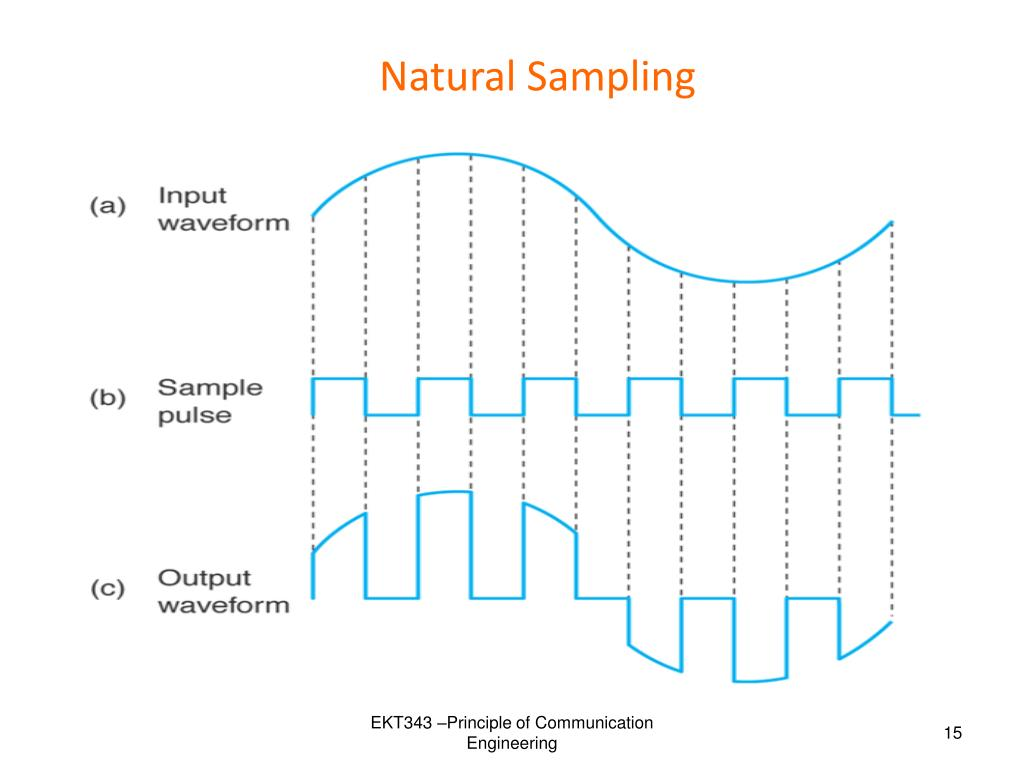
\includegraphics[width=0.7\linewidth]{../Ejercicio-3/ImagenesEjercicio3/natural-sampling1-l}
	\caption{Muestreo Natural con llave analogica}
	\label{fig:natural-sampling1-l}
\end{figure}

En el domino de las frecuencias el tren de pulsos es representado por una \textbf{sinc discreta}. El espectro resultante se ilustra en la siguiente imagen
	
\begin{figure}[H]
	\centering
	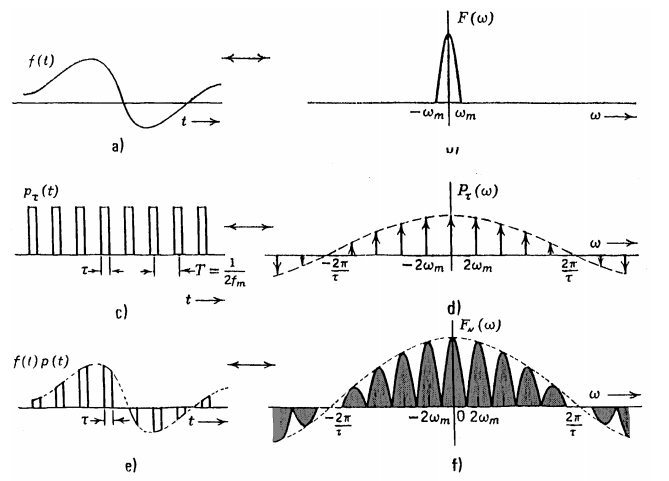
\includegraphics[width=0.7\linewidth]{../Ejercicio-3/ImagenesEjercicio3/Espectro}
	\caption{Espectro resultante de utilizar al utiliza la llave analogica}
	\label{fig:espectro}
\end{figure}

Si el tiempo de apertura de la llave se reduce entonces obtendremos una envolvente más aplanada. Esto reduce los efectos de distorsión introducidos por la forma de la sinc.

